\documentclass[12pt]{article}

% Packages
\usepackage[utf8]{inputenc}
\usepackage{graphicx}
\usepackage{hyperref}
\usepackage{enumitem}

\usepackage[backend=biber,style=authoryear,citestyle=authoryear,natbib=true]{biblatex}
\addbibresource{references_india.bib}
\usepackage[a4paper, margin=0.8in]{geometry}
\usepackage{titlesec}
\setlength{\parskip}{1em} 
\setlength{\bibitemsep}{1em} % Add spacing between bibliography entries

%Customizing section titles
% Customize section and subsection titles
\titleformat{\section}
  {\normalfont\Large\bfseries} % Section titles will be in large, bold font
  {\thesection}{1em}{}
%   \titlespacing{\subsection}{0pt}{*0}{-0.8em}
  [\titlerule]
  
%Italicised subsectiom
\titleformat{\subsection}
  {\normalfont\bfseries\itshape} % Subsection titles will be slightly smaller
  {\thesubsection}{1em}{}
\titlespacing{\subsection}{0pt}{0em}{-0.3em}

% Regular non-italic subsection (unnumbered)
\newcommand{\regularsubsection}[1]{%
  \vspace{1em} % Adjust spacing if needed
  \noindent\textbf{#1}\par\vspace{-0.3em}}

% Title
\title{Adaptation Plan Evaluation Report}
\author{Mukund Balaji Srinivas | u7274095}
\date{} % Remove the date 

\begin{document}

% Title Page
\maketitle

\begin{abstract}
This section provides a brief summary of the evaluation report, outlining the key question being addressed, methods used, 
and main conclusions.
\end{abstract}

\newpage

\section*{Introduction}
Climate change in India affects multiple facets of the ecosystem, including oceans (\cite{marathe_2021}).
coastal regions (\cite{gupta_2019}), water resources (\cite{shiva_shankar_2021}) and forests (\cite{Lele2019ClimateCA}). Additionally, it significantly impacts 
agriculture (\cite{Kumar2023DeterminantsOC}), urban areas, public health(\cite{rajput_2022}), and energy infrastructure (\cite{Yarlagadda_22}), 
creating complex challenges that require coordinated responses. For this report, we will focus on adaptation measures in three key sectors: water resources, coastal regions, and public health.
\subsection*{Coastal Regions}
Climate change is projected to exacerbate the impacts of tropical cyclonic storms by increasing their intensity as sea surface temperatures 
rise. The North Indian Ocean comprising the Bay of Bengal and the Arabian Sea accounts for only 7\% of global cyclones 
these storms are disproportionately destructive, particularly along the densely populated, low-lying East Indian and Bangladeshi coasts, 
which are highly vulnerable to storm surges and flooding. Also, while the Arabian Sea has historically experienced fewer high-intensity storms due to 
factors such as unfavourable wind shear, dry air from the Thar Desert, and cooler sea temperatures, recent years have seen a rise in stronger cyclones 
in the region. This shift suggests that changing climatic conditions are altering traditional storm patterns and intensifying their impacts, posing 
new challenges for coastal resilience and disaster preparedness (\cite{gupta_2019})

\subsection*{Water resources}
Climate change poses a significant threat to water, food security, and the well-being of India’s 
1.2 billion people in the 21st century . The country experiences uneven spatial distribution of water resources, 
with the drier northwest receiving scarce rainfall, while the northeast holds the distinction of being the 
wettest region on Earth (\cite{goyal_2018}). Agriculture supports 17.2\% of the global population 
despite relying on just 9\% of the world's arable land, with more than 56\% of agricultural land being rainfed (\cite{goyal_2018}). 

This heavy dependence on rainfall makes India particularly vulnerable to climate variability. Precipitation patterns are expected 
to shift significantly, with projections showing an increase in average annual rainfall by 7-18.7\% by 2099 compared to the 1961-1990 baseline (\cite{chaturvedi_2012}).
Similarly, precipitation in several river basins across India could increase by up to 30\% by 2040-2069 and 50\% by 2070-2099 from the 1971-2005 levels (\cite{mishra_2016}).
The A1B (\cite{ipcc_2000}) scenario further projects higher precipitation, particularly in southern India (\cite{kim_2009}). In the Brahmaputra basin, premonsoon rainfall is expected 
to rise by approximately 100 mm by 2071-2100, compared to the 1961-1990 baseline (\cite{ghosh_2012}).With India’s agrarian economy being heavily dependent on monsoons and water 
availability, these projected changes pose serious risks to agricultural productivity and food security, increasing the vulnerability of millions of livelihoods (\cite{goyal_2018})



\pagebreak

\regularsubsection{Adaptation Policy and activities}
The National Action Plan on Climate Change [NAPCC] (\cite{napcc_2008}) articulates India's adaptation goals addressing climate 
vulnerabilities across key sectors while promoting sustainable growth. NAPCC identifies eight National Missions, which form 
the core of the National Action Plan, out of which five missions are focusing on adaptation, which are:
\begin{enumerate}
  \item \textbf{National Water Mission}: Promotes integrated water resource management to conserve water, minimize wastage, 
  and ensure equitable distribution across regions and states.  
  \item \textbf{Mission for Sustaining the Himalayan Ecosystem}: Aims to safeguard Himalayan glaciers and ecosystems through 
  sustainable management and a monitoring network.  
  \item \textbf{National Mission for a Green India}: Focuses on enhancing ecosystem services, including carbon sequestration, 
  through afforestation and reforestation efforts.
  \item \textbf{National Mission for Sustainable Agriculture}: Seeks to build climate resilience in agriculture by adopting new 
  technologies, integrating traditional knowledge, and introducing improved credit and insurance systems. 
  \item \textbf{National Mission on Strategic Knowledge for Climate Change}: Facilitates research, innovation, 
  and global collaboration to address climate challenges and develop effective responses.
\end{enumerate}

\begin{figure}[h]
  \centering
  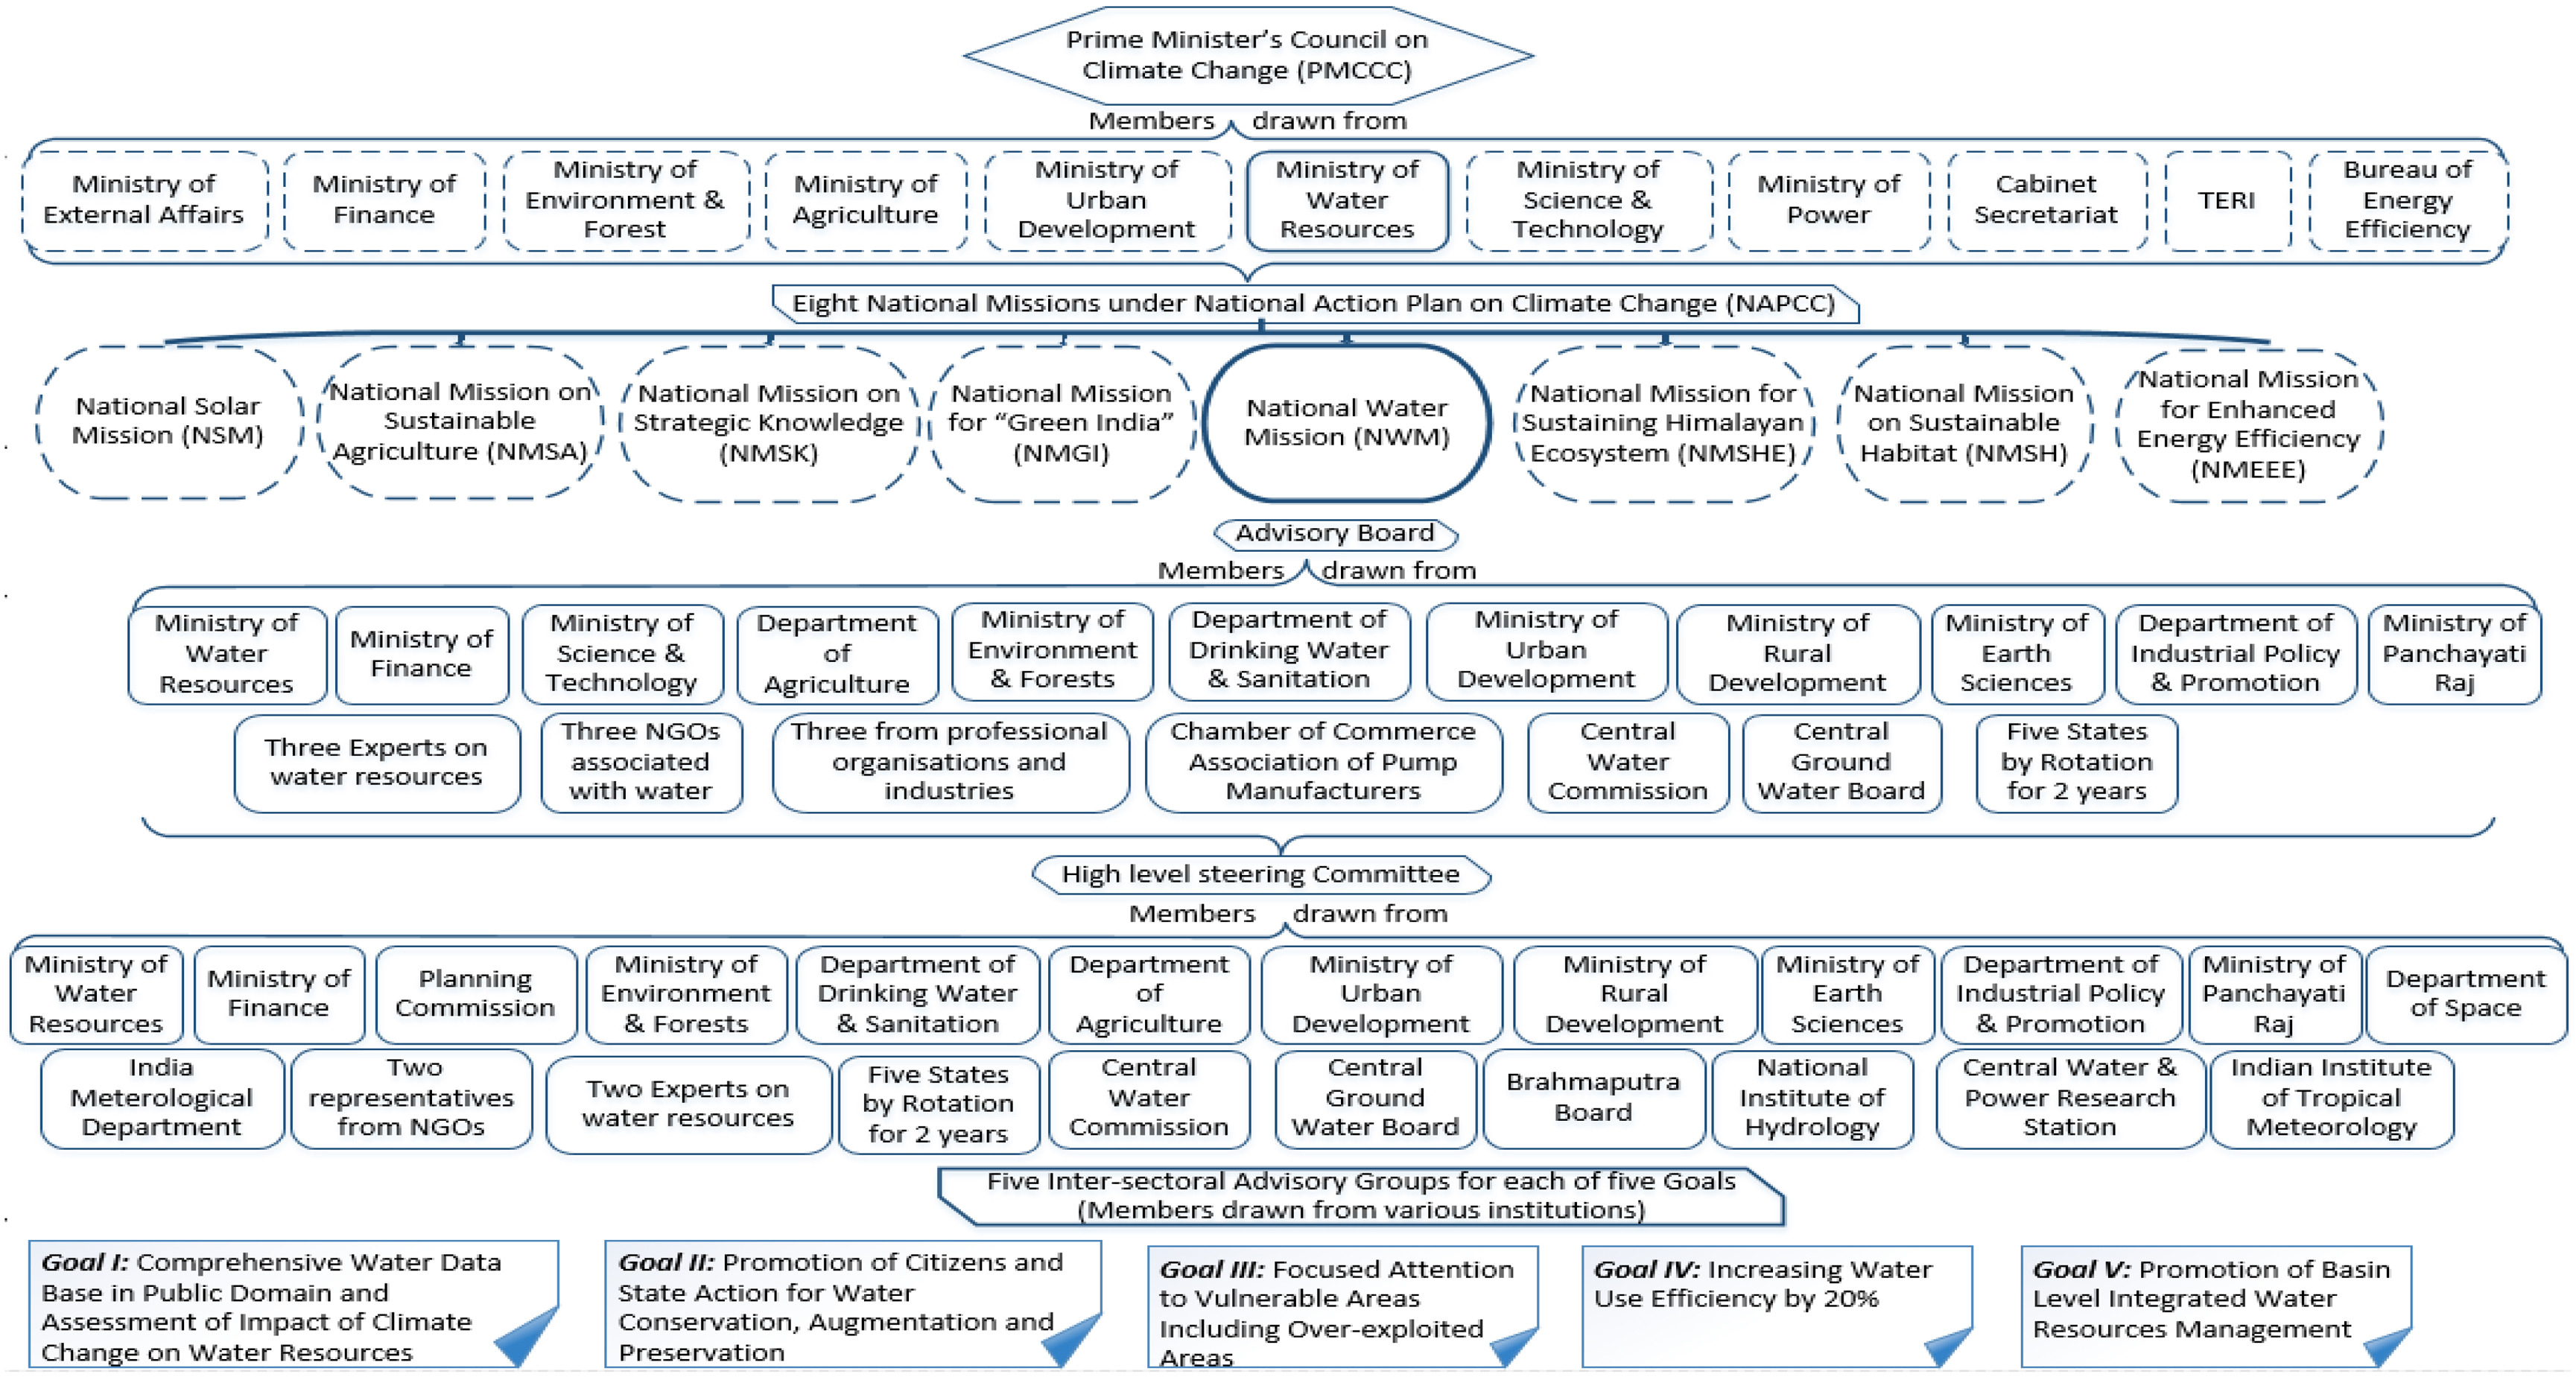
\includegraphics[width = \textwidth]{NAPCC_india.jpg}
  \caption{Institutions involved in the National Action Plan on Climate Change. (\cite{azohani_2017})}
\end{figure}




\section*{Methods}
\subsection*{Water Resources}
The analysis will evaluate whether the key adaptations implemented under the National Water Mission (\cite{napcc_2008}).
SSAP (\cite{SSAP_2015}) or other institutions such as the Atal Bhujal Yojana (\cite{nandakumaran_2020}) align with 
global recommendations outlined by the IPCC recommendations (\cite{ipcc_climate_2023}).Additionally, the analysis will 
explore whether these institutions share a consistent understanding of risk with the IPCC’s framework, The IPCC identifies 
the disproportionate impacts on vulnerable populations and highlights the critical importance of adaptive water management. 
This comparison will help determine if the institutions' adaptation strategies are aligned not only in their objectives but 
also in their risk perceptions and frameworks for action.

The IPCC-recommended adaptation measures for water management include rainwater harvesting, soil moisture conservation, 
and supportive public policies (\cite{ipcc_climate_2023} , TS.D.5.1, 5.2,5.8).This report will assess the extent to 
which these measures are integrated into national and state-level strategies. The assessments will be summarised in 
a tabular format as recommended by (\cite{craft_2016})



\section*{Assesment}


\end{document}
